\documentclass{article}
%%%%%%%%%%%%%%%%%%%%%%%%%%%%%%%%%%%%%%%%%%%%%%%%%%%%%%%%%%%%%
% Lecture Specific Information to Fill Out
%%%%%%%%%%%%%%%%%%%%%%%%%%%%%%%%%%%%%%%%%%%%%%%%%%%%%%%%%%%%%
\newcommand{\LectureTitle}{Lecture \#2 Notes}
%\newcommand{\LectureDate}{\today}
\newcommand{\LectureDate}{August\ 30,\ 2011}
\newcommand{\LectureClassName}{CHE\ 858}
\newcommand{\LatexerName}{Miguel\ Wong}
%%%%%%%%%%%%%%%%%%%%%%%%%%%%%%%%%%%%%%%%%%%%%%%%%%%%%%%%%%%%%

% Change "article" to "report" to get rid of page number on title page
\usepackage{amsmath,amsfonts,amsthm,amssymb}
\usepackage{setspace}
\usepackage{Tabbing}
\usepackage{fancyhdr}
\usepackage{lastpage}
\usepackage{extramarks}
\usepackage{chngpage}
\usepackage{soul,color}
\usepackage{graphicx,float,wrapfig}
\usepackage{afterpage}
\usepackage{abstract}
\usepackage[version=3]{mhchem} % for chemical equations
\usepackage{chemfig} % for drawing chemical compounds
\usepackage{pgfplots} % for plotting equations

% In case you need to adjust margins:
\topmargin=-0.45in
\evensidemargin=0in
\oddsidemargin=0in
\textwidth=6.5in
\textheight=9.0in
\headsep=0.25in

% Setup the header and footer
\pagestyle{fancy}
\lhead{\LatexerName}
\chead{\LectureClassName: \LectureTitle}
\rhead{\LectureDate}
\lfoot{\lastxmark}
\cfoot{}
\rfoot{Page\ \thepage\ of\ \pageref{LastPage}}
\renewcommand\headrulewidth{0.4pt}
\renewcommand\footrulewidth{0.4pt}

%%%%%%%%%%%%%%%%%%%%%%%%%%%%%%%%%%%%%%%%%%%%%%%%%%%%%%%%%%%%%
% Some tools
\newcommand{\enterTopicHeader}[1]{\nobreak\extramarks{#1}{#1 continued on next page\ldots}\nobreak
                                    \nobreak\extramarks{#1 (continued)}{#1 continued on next page\ldots}\nobreak}
\newcommand{\exitTopicHeader}[1]{\nobreak\extramarks{#1 (continued)}{#1 continued on next page\ldots}\nobreak
                                   \nobreak\extramarks{#1}{}\nobreak}

\newlength{\labelLength}
\newcommand{\labelAnswer}[2]
  {\settowidth{\labelLength}{#1}
   \addtolength{\labelLength}{0.25in}
   \changetext{}{-\labelLength}{}{}{}
   \noindent\fbox{\begin{minipage}[c]{\columnwidth}#2\end{minipage}}
   \marginpar{\fbox{#1}}

   % We put the blank space above in order to make sure this
   % \marginpar gets correctly placed.
   \changetext{}{+\labelLength}{}{}{}}

\setcounter{secnumdepth}{0}
\newcommand{\TopicName}{}
\newcounter{TopicCounter}
\newenvironment{Topic}[1][Problem \arabic{TopicCounter}]
  {\stepcounter{TopicCounter}
   \renewcommand{\TopicName}{#1}
   \section{\TopicName}
   \enterTopicHeader{\TopicName}}
  {\exitTopicHeader{\TopicName}}
  
\setcounter{secnumdepth}{0}
\newcommand{\ExampleSectionName}{}
\newcounter{ExampleSectionCounter}[TopicCounter]
\newenvironment{ExampleSection}[1][Example \arabic{ExampleSectionCounter}]
  {\stepcounter{ExampleSectionCounter}
   \renewcommand{\ExampleSectionName}{#1}
   \section{\ExampleSectionName}
   \enterTopicHeader{\ExampleSectionName}}
  {\exitTopicHeader{\ExampleSectionName}}

\setcounter{secnumdepth}{0}
\newcounter{ExampleBoxCounter}[TopicCounter]
\newcommand{\examplebox}[1]
  {
  % We put this space here to make sure we're disconnected from the previous
   % passage
   \stepcounter{ExampleBoxCounter}
   \noindent\fbox{\begin{minipage}[c]{\columnwidth}#1\end{minipage}}\enterTopicHeader{\ExampleSectionName}\exitTopicHeader{\ExampleSectionName}\marginpar{\fbox{\#\arabic{ExampleBoxCounter}}}
   % We put the blank space above in order to make sure this
   % \marginpar gets correctly placed.
   \vskip10pt
   }

\renewcommand{\contentsname}{{\normalsize Topics Covered}}
\renewcommand{\abstractname}{\LectureTitle\ Summary}
\renewcommand{\absnamepos}{flushleft}

%%%%%%%%%%%%%%%%%%%%%%%%%%%%%%%%%%%%%%%%%%%%%%%%%%%%%%%%%%%%%

\begin{document}
\begin{spacing}{1.1}
\newpage

\begin{abstract}
This is a fun example of the notes that can be taken within this template. 
\end{abstract}

\tableofcontents
\addtocontents{toc}{~\hfill\textbf{Page}\par}
\vskip10pt
\hrule
\vskip10pt

% When topics are long, it may be desirable to put a \newpage or a
% \clearpage before each Topic environment
%\newpage
\begin{Topic}[Chemistry \Roman{TopicCounter}]
Let's make some salt to start: \ce{SO4^2- + Ba^2+ -> BaSO4 v}
\end{Topic}

\begin{Topic}[Chemistry \Roman{TopicCounter}]
Now how about some organic chemistry?

\begin{ExampleSection}
Remember Fischer Esterifications? No? Here is a not so great reminder! \\

\examplebox{
In Fischer Esterifications we want to make something like this:\\

\chemfig{*6((-MeO)=(-OMe)-=(-(-[:-30]O-[:30]-[:0](-[:60])-[:-60])=[:90]O)-=(-MeO)-)}
}
\end{ExampleSection}

\end{Topic}


\begin{Topic}[Mathematics \& Statistics]
Aliquam erat volutpat. Vivamus dictum volutpat urna. Sed tempor
interdum sapien. Cras id mi in nunc aliquet placerat. Maecenas
gravida accumsan ipsum. Integer nec elit vitae ligula pretium
tincidunt. Sed libero metus, condimentum vel, suscipit et, varius
id, mi. Nunc accumsan pharetra leo. Pellentesque et est quis tellus
adipiscing scelerisque. Mauris lacinia erat quis nulla. Nunc
vulputate. Cras pretium libero sed elit. Sed lectus. Cras mauris
odio, ullamcorper a, dictum non, mattis id, urna. Suspendisse sed
ligula.
\begin{ExampleSection}
\examplebox{
When life was still Gaussian.

\begin{displaymath}
f(x) = ae^{\frac{(x-b)^{2}}{2c^{2}}}
\end{displaymath}

You can also highlight parts of an equation too!

\begin{displaymath}
f(x) = ae^{\frac{\textcolor{red}{(x-b)^{2}}}{2c^{2}}}
\end{displaymath}
}
\end{ExampleSection}

\begin{ExampleSection}
\examplebox{
\newcommand\gauss[2]{1/(#2*sqrt(2*pi))*exp(-((x-#1)^2)/(2*#2^2))} % Gauss function, parameters mu and sigma

\begin{tikzpicture}
\begin{axis}[every axis plot post/.append style={
  mark=none,domain=-2:3,samples=50,smooth}, % All plots: from -2:2, 50 samples, smooth, no marks
axis x line*=bottom, % no box around the plot, only x and y axis
axis y line*=left, % the * suppresses the arrow tips
enlargelimits=upper] % extend the axes a bit to the right and top
\addplot {\gauss{0}{0.5}};
\addplot {\gauss{1}{0.75}};
\end{axis}
\end{tikzpicture}
}
\end{ExampleSection}
\end{Topic}

\begin{Topic}[Simple Economics]
\begin{ExampleSection}
\examplebox{
Skyrocketing supply! \\

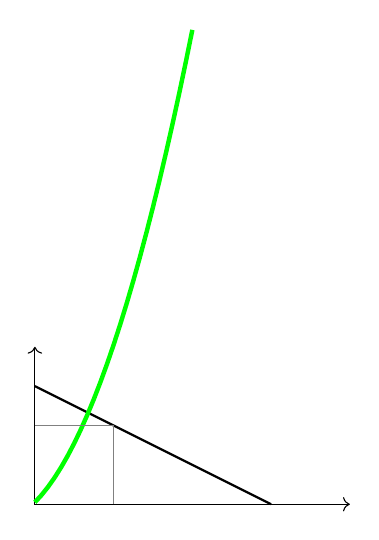
\begin{tikzpicture}
\draw [<->] (0,2) -- (0,0) -- (4,0);
\draw [thick] (0,1.5) -- (3,0);
\draw[green, ultra thick, domain=0:2.0] plot (\x, {0.025+\x+\x*\x});
\draw [help lines] (1,0) -- (1,1) -- (0,1);
\end{tikzpicture}
}
\end{ExampleSection}
\end{Topic}

\newpage
\begin{Topic}[Now, To $\infty$ and Beyond\ldots]
Aliquam erat volutpat. Vivamus dictum volutpat urna. Sed tempor
interdum sapien. Cras id mi in nunc aliquet placerat. Maecenas
gravida accumsan ipsum. Integer nec elit vitae ligula pretium
tincidunt. Sed libero metus, condimentum vel, suscipit et, varius
id, mi. Nunc accumsan pharetra leo. Pellentesque et est quis tellus
adipiscing scelerisque. Mauris lacinia erat quis nulla. Nunc
vulputate. Cras pretium libero sed elit. Sed lectus. Cras mauris
odio, ullamcorper a, dictum non, mattis id, urna. Suspendisse sed
ligula.\\

\examplebox{Vestibulum tortor. Etiam sagittis purus quis nisl. Vestibulum vitae
dui vitae wisi faucibus molestie. Cum sociis natoque penatibus et
magnis dis parturient montes, nascetur ridiculus mus. Sed tincidunt
risus eu leo. Quisque bibendum eros et erat. Proin lobortis nunc.
Praesent vel justo eget odio mattis aliquet. Curabitur ultricies
ante id eros. Nulla vehicula arcu sit amet ipsum. Proin sodales odio
at justo. Vestibulum ante ipsum primis in faucibus orci luctus et
ultrices posuere cubilia Curae; Pellentesque habitant morbi
tristique senectus et netus et malesuada fames ac turpis egestas.
Praesent venenatis. Integer justo.}
\end{Topic}

\end{spacing}
\end{document}